\documentclass[letterpaper,spanish]{article}
\usepackage{babel}
\usepackage[latin1]{inputenc}
\usepackage[pdftex]{graphicx}
\usepackage[dvipsnames,usenames]{color}
\usepackage{fancyhdr}
\usepackage{latexsym}

\oddsidemargin -0.3cm \topmargin -1.1cm \headheight 2.5cm
\textwidth 16.8cm \textheight 19.8cm

\newsavebox{\fondo}
\sbox{\fondo}{
\includegraphics[keepaspectratio,height=1.35\textheight,width=1.35\textwidth]{../../02_publicimage/margin.png}}

\pagestyle{fancy}
\fancyhead[C]{\setlength{\unitlength}{1in}
\begin{picture}(0,0)\put(-3.9,-9.3){\usebox{\fondo}}\end{picture}}

\renewcommand{\headrulewidth}{0pt}
\title{\huge{\textbf{DOCUMENTO DE DISE�O \\ Componentes de gesti�n de usuarios y autentificaci�n}}}
\author{Yeah! S.R.L.}
\date{\small{20 de marzo 2009}}

\begin{document}
\maketitle \pagebreak \tableofcontents \pagebreak

\section{INTRODUCCION}

Basados en el documento de analisis, se presentan los siguientes modelos de la solucion propuesta.

\section{CASOS DE USO}

\begin{center}
    \includegraphics[width=1.00\textwidth]{images/usecase_category.png}
    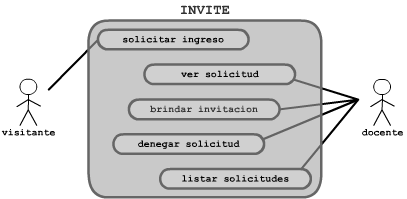
\includegraphics[width=1.00\textwidth]{images/usecase_invite.png}
    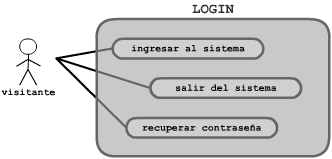
\includegraphics[width=1.00\textwidth]{images/usecase_login.png}
    \includegraphics[width=1.00\textwidth]{images/usecase_role.png}
    \includegraphics[width=1.00\textwidth]{images/usecase_user.png}
\end{center}

\section{MODELO DE DATOS}

\begin{center}
    \includegraphics[width=1.00\textwidth]{images/relationalmodel.png}
\end{center}

\section{MODELO DE NAVEGACION}

\begin{center}
    \includegraphics[width=1.00\textwidth]{images/navegationmodel.png}
\end{center}

\vspace{0.5cm}

Le�do el presente documento, fu� revisado por un representante de la empresa TIS, juntamente con el representante de la grupo-empresa Yeah S.R.L., el director del proceso de analisis y sus colaboradores. Encontrandose las siguientes observaciones:

\vspace{0.5cm}

\begin{verbatim}
.........................................................................................
.........................................................................................
.........................................................................................
.........................................................................................
.........................................................................................
.........................................................................................
.........................................................................................
.........................................................................................
.........................................................................................
.........................................................................................
.........................................................................................
.........................................................................................
\end{verbatim}


\vspace{1.5cm}
    \begin{table}[htbp]
        \begin{center}
            \begin{tabular}{c c}
\_\_\_\_\_\_\_\_\_\_\_\_\_\_\_\_\_\_\_\_\_\_\_\_\_\_\_\_\_\_\_\_\_\_\_\_\_\_\_\_\_\_\_ &
\_\_\_\_\_\_\_\_\_\_\_\_\_\_\_\_\_\_\_\_\_\_\_\_\_\_\_\_\_\_\_\_\_\_\_\_\_\_\_\_\_\_\_ \\
Lic. Leticia Blanco Coca & Luis Arce Claros \\
Representante legal de la empresa TIS & Director del proceso de analisis de la empresa Yeah! S.R.L.\\
            \end{tabular}
        \label{tab1}
        \end{center}
    \end{table}

\end{document}
